\section{Organiser ses données}
\subsection{Les fichiers : noms et contenu}
\begin{frame}{Un fichier}
  \begin{block}{De l'information au stockage}
    Les informations utilisées dans un ordinateur sont stockées dans la
    \emph{mémoire de masse}, qui se distingue de la \emph{mémoire vive}
    par sa résistance à l'extinction et de la \emph{mémoire morte} (et
    plus tard, du \emph{firmware}) par sa mutabilité.

    Les performances des systèmes de stockage de masse sont meilleures
    chaques années, mais l'ordre de grandeur reste la ms ou 100 µs.
  \end{block}
  \begin{block}{De l'information au fichier}
    L'information est découpée en petites unités qui s'appellent des
    fichiers, sémantiquement cohérentes --- ce sont des informations qui
    « vont ensemble ». Ces éléments de base du stockage informatique
    peuvent ne contenir que très peu d'information ou représenter
    plusieurs Go de données par fichier.

    Un fichier est lié à la façon dont on y accède (son \emph{nom} et
    son \emph{chemin}), mais nous verrons que ce n'est pas un
    identifiant : il peut y avoir plusieurs accès différents à un même
    fichier (\emph{liens}).
  \end{block}
\end{frame}
\begin{frame}{Noms et contenu des fichiers}
  \begin{block}{La décomposition traditionnelle d'un nom de fichier}
    \begin{columns}
      \begin{column}{8cm}
        Deux parties séparées par un point:
        \begin{itemize}
        \item La $1\up{ère}$ partie informe sur la nature du contenu du
          fichier,
        \item La $2\up{ème}$ partie informe sur le format ou la finalité des données.
        \end{itemize}
      \end{column}
      \begin{column}{3cm}
        \begin{tabular}{|r@{}r@{}l|}
          \hline
          {\color{solarizedRed}nom}&.&{\color{solarizedGreen}extension} \\
          {\color{solarizedRed}prefix}&.&{\color{solarizedGreen}suffix} \\
          {\color{solarizedRed}description}&.&{\color{solarizedGreen}format}\\
          \hline
        \end{tabular}
      \end{column}
    \end{columns}
    \begin{itemize}
    \item[\ddialogwarning] Selon les systèmes, certains caractères sont interdits. Par exemple \texttt{*} sous Windows, \texttt{/} sous Linux.
    \end{itemize}
  \end{block}
  \begin{columns}
    \begin{column}{5.5cm}
      \begin{block}{Exemples de noms de fichiers}
        \begin{center}
          \begin{tabular}{ll}
            \hline
            Extension&Contenu\\
            \hline
            .c&Sources C\\
            .html&Document Web\\
            .pdf&Document Mis en page\\
            .txt&Texte brut\\
            \hline
          \end{tabular}
          \vfill
          \begin{tabular}{ll}
            \hline
            Enigmatique&Informatif\\
            \hline
            e3.c&teste\_boucle\_for.c\\
            New.pdf&2011\_IntroSys\_cours\_1.pdf\\
            toto.sh&test\_boucle\_for.sh\\
            \hline
          \end{tabular}
        \end{center}
      \end{block}
    \end{column}
    \begin{column}{5.5cm}
      \begin{alertblock}{Choix des noms}
        \begin{itemize}
        \item[\ddialoginformation] Ils doivent être choisis minutieusement pour être informatifs.
        \item[\ddialogsystem] Choisir un nom : réfléchir pour un gain de temps pour
          retrouver le fichier ou le répertoire concerné.
        \item[\ddialogwarning] Importance de la casse (Linux), tolérance
          ailleurs (OS X, Windows).
        \end{itemize}
      \end{alertblock}
    \end{column}
  \end{columns}
\end{frame}
\subsection{Organisation des données enregistrées}
\begin{frame}{Des fichiers et des répertoires}
  \begin{block}{Les fichiers... en vrac ?}
    Les fichiers sont regroupés dans des répertoires (en anglais
    \emph{directory} ou \emph{folders}). Les répertoires peuvent
    contenir des fichiers ou d'autres répertoires. L'organisation des
    fichiers est réglée par le \emph{système de fichiers}
    (ang. \emph{filesystem}).

    \begin{itemize}
    \item Cette organisation arborescente permet de faciliter la
      recherche d'un fichier,
    \item Les fichiers sont regroupés par application, par thème, par
      format, par fonction, \dots
    \item Organisation \emph{hiérarchique} qui permet d'organiser les données et
      de faciliter leur accès.
    \end{itemize}
  \end{block}
  \begin{columns}
    \begin{column}{.7\linewidth}
      \begin{block}{De très nombreux fichiers et répertoires}
        \begin{itemize}
        \item[\ddialoginformation] Le nombre de fichiers enregistrés sur un disque dur peut
          aisément dépasser 100.000 fichiers,
        \item Dans un même répertoire le nom est un identifiant.
        \item Les répertoires et les fichiers partagent les mêmes noms.
        \item[\dialogwarning] Sous Windows, pas d'extension pour les répertoires.
        \end{itemize}
      \end{block}
    \end{column}%
    \begin{column}{.25\linewidth}
      % 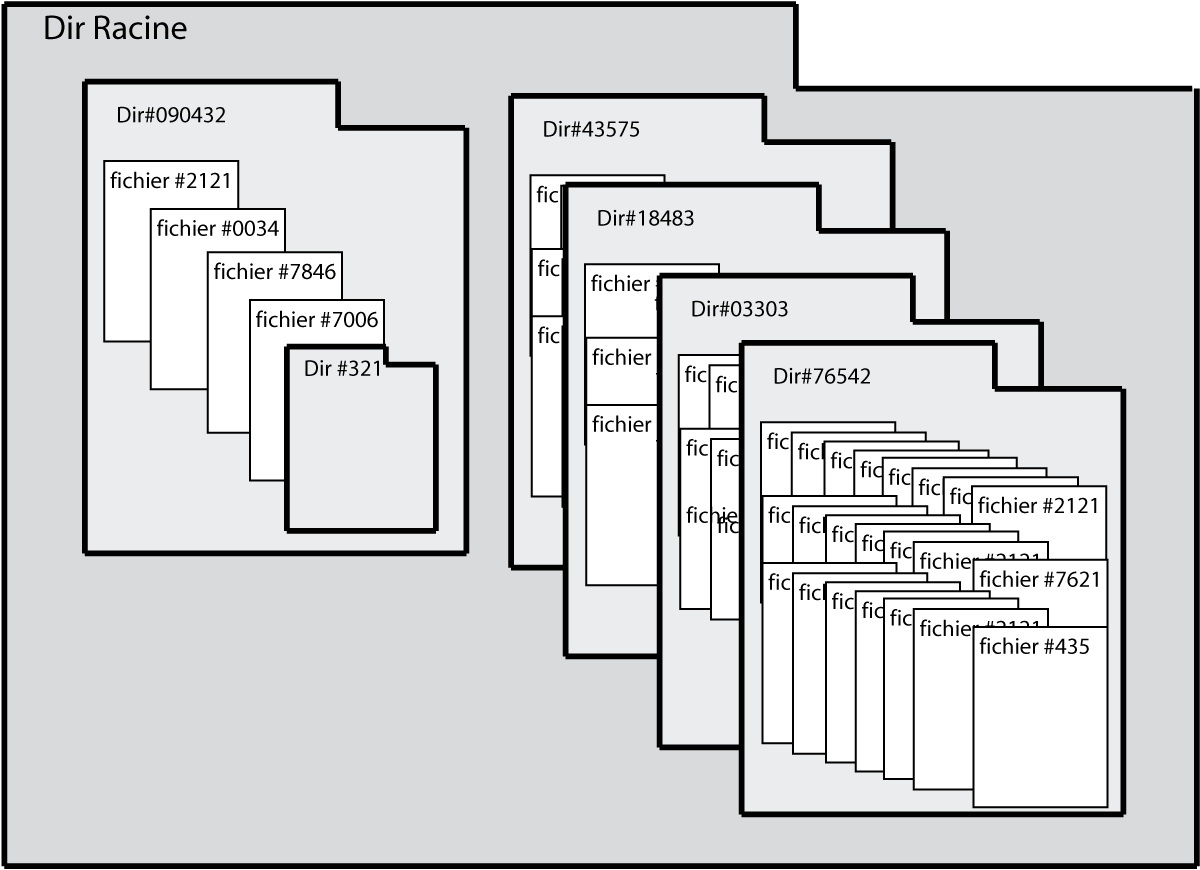
\includegraphics[width=\linewidth]{img/s02/file_system}
      \begin{alertblock}{Remarque}
        \begin{itemize}
        \item[\dialogerror] Avec tous les fichiers au même
          \textit{endroit}, il est très difficile de les lister (trop à
          lire).
        \end{itemize}
      \end{alertblock}
    \end{column}
  \end{columns}
\end{frame}

\subsection{L'organisation arborescente}
\begin{frame}{Exemple d'arborescence Linux}
  \dirtree{%
    .1 \DTd{}\DTfcomment{Répertoire racine \emph{(Root Directory)}}.  .2
    \DTd{bin}.  .3 (\dots).  .2 \DTd{home}.  .3
    \DTd{moi}\DTfcomment{Répertoire personnel \emph{(User
        directory)}}.  .4 \DTd{Mes~Documents}.  .5 ListeDesCourses.txt.
    .5 Exercice\_1.sh.  .4 (\dots).  .3 \DTd{anonymous}.  .4
    LisezMoi.txt.  .4 \DTd{Telechargements}.
    % .5 Cours\_Systeme.pdf.
    .5 (\dots).  .2 (\dots).  }
  \begin{alertblock}{Les répertoires importants}
    \begin{itemize}
    \item La \textbf{racine} (\textit{Root directory}) contient tous
      les répertoires et fichiers accessibles depuis le système.
    \item Le \textbf{répertoire personnel} (\textit{User Directory} ou
      \textit{Home Directory}) est le répertoire dans lequel
      l'utilisateur peut faire ce qu'il veut (écrire, modifier,
      supprimer, installer \dots).
    \end{itemize}
  \end{alertblock}
\end{frame}
\subsection{La notion de chemin}
\begin{frame}{La notion de chemin}
  \begin{block}{Le chemin définit un accès unique à partir de la racine}
    \begin{itemize}
    \item Deux fichiers ou répertoires ne peuvent pas porter le même nom
      si ils sont dans un même répertoire.
    \item Sous Linux, les noms des fichiers et répertoires différencient
      les caractères \textsc{Majuscules} et minuscule. Les fichiers
      \alert{E}ssai.txt et \alert{e}ssai.txt peuvent donc être dans le
      même répertoire.
    \end{itemize}
  \end{block}
  \begin{block}{Exemples de chemins absolus}
    \dirtree{%
      .1 \DTd{}\DTfcomment{Un chemin absolu part de la racine {\color{solarizedAccent}/}}.
      .2 \DTd{home}\DTfcomment{/{\color{solarizedAccent}home/}}.
      .3 \DTd{moi}\DTfcomment{/home/{\color{solarizedAccent}moi/}}.
      .4 \DTd{Etoiles}\DTfcomment{/home/moi/{\color{solarizedAccent}Etoiles/}}.
      .5 SOLEIL.jpg\DTfcomment{/home/moi/Etoiles/{\color{solarizedAccent}SOLEIL.jpg}}.
      .5 Soleil.jpg\DTfcomment{/home/moi/Etoiles/{\color{solarizedAccent}Soleil.jpg}}.
      .4 \DTd{Systeme\_Solaire}\DTfcomment{/home/moi/{\color{solarizedAccent}Systeme\_Solaire/}}.
      .5 SOLEIL.jpg\DTfcomment{/home/moi/Systeme\_Solaire/{\color{solarizedAccent}SOLEIL.jpg}}.
    }
  \end{block}
  \begin{alertblock}{Syntaxe d'un chemin absolu}
    Le chemin \textit{absolu} d'un élément du système de fichier est
    unique (sauf avec un \emph{lien}). Il donne la liste des répertoires
    et sous-répertoires en partant de la racine \lin{/} (la référence de
    l'arborescence) jusqu'à la cible.
  \end{alertblock}
\end{frame}

% MOVE TO 03
% \begin{frame}{La notion de partition}
%   \begin{block}{Windows : les partitions visibles}
%     Le ou les disques sont découpés en systèmes de fichiers indépendants
%     qui sont numérotés par des lettres. A et B sont réservés au lecteur
%     de disquette, C au disque système. Nombre limité de partitions.

%     Les partitions aident à l'organisation des données par type
%     (système, utilisateurs, sauvegarde).
%   \end{block}
%   \begin{block}{Unix : les partitions invisibles}
%     Sous Unix et ses variantes (OS X et Linux), la partition racine est
%     celle qui contient le système. Les autres partitions sont
%     \emph{montées} à la place d'un répertoire et sont en quelque sortes
%     greffées dans l'arbre qui reste unique. La racine de la partition
%     montée prend la place du répertoire dans l'arborescence.
%   \end{block}
% \end{frame}

\subsection{Répertoire courant et chemins relatifs}
\begin{frame}{Répertoire courant et chemins relatifs}
  \begin{block}{Le répertoire courant}
    \begin{itemize}
    \item Le répertoire courant est un répertoire de référence d'où sont
      lancées les commandes du shell.
    \item Par défaut, le répertoire courant est le répertoire personnel
      de l'utilisateur,
    \item Naviguer dans l'arborescence équivaut à modifier le répertoire
      courant.
    \end{itemize}
  \end{block}
  \begin{block}{Exemples de chemins relatifs}
    \dirtree{%
      .1 \DTd{home}\DTfcomment{../..}.
      .2 \DTd{moi}\DTfcomment{../}.
      .3 \DTd{Etoiles}\DTfcomment{{\color{solarizedRed}Répertoire Courant ~~./}}.
      .4 SOLEIL.jpg\DTfcomment{SOLEIL.jpg {\color{black}ou} ./SOLEIL.jpg}.
      .4 Antares.jpg\DTfcomment{Antares.jpg {\color{black}ou} ./Antares.jpg}.
      .3 \DTd{Systeme\_Solaire}\DTfcomment{../Systeme\_Solaire/}.
      .4 terre.gif\DTfcomment{../Systeme\_Solaire/terre.gif}.
    }
  \end{block}
  \begin{alertblock}{Syntaxe d'un chemin relatif}
    \begin{itemize}
    \item Le chemin \textit{relatif} d'un fichier ou d'un répertoire donne la liste des répertoires et sous-répertoires en partant du répertoire courant (la référence \textit{relative} dans l'arborescence) jusqu'à la cible.
    \item Il est relatif, car lorsque le répertoire courant change, le chemin relatif change.
    \end{itemize}
  \end{alertblock}
\end{frame}
% MOVE TO 03
% \begin{frame}{Chemin canonique}
%   \begin{block}{Chemin canonique}
%     Le chemin qui part de la racine et n'emprunte aucun \emph{lien symbolique} (une forme de lien que nous verrons plus loin) ni aucun \emph{lien parent} (raccourci \lin{..} vers un répertoire parent d'un autre) est appelé le chemin \emph{canonique absolu}.
%   \end{block}
% \end{frame}
%%%%%%%%%%%%%% 
\subsection{Notation spéciales}
\begin{frame}{Notation spéciales}
  \begin{block}{Les chemins des répertoires de référence}
    \begin{columns}
      \begin{column}{6cm}
        \begin{center}
          \begin{tabular}{lr}
            \hline
            Répertoire&Notation\\
            \hline
            Répertoire racine&\lin{/}\\
            Répertoire personnel&\lin{\~{}}\\
            \hline
          \end{tabular}
        \end{center}
      \end{column}
      \begin{column}{6cm}
        \begin{center}
          \begin{tabular}{lr}
            \hline
            Répertoire&Notation\\
            \hline
            Répertoire courant&\lin{.}\\
            Répertoire parent&\lin{..}\\
            \hline
          \end{tabular}
        \end{center}
      \end{column}
    \end{columns}
    \begin{itemize}
    \item[\ddialogwarning] La notation \lin{\~{}} est un chemin
      absolu, remplacée par le vrai chemin avant l'exécution des
      commandes. C'est un raccourci \emph{au niveau du shell, pas au
        niveau du système d'exploitation}.
    \end{itemize}
  \end{block}
  \begin{block}{Exemple de chemins valides pointant le fichier cible}
    \begin{columns}
      \begin{column}{55mm}
        \dirtree{%
          .1 \DTd{}\DTfcomment{{\color{solarizedAccent}Répertoire Racine}}.
          .2 \DTd{home}.
          .3 \DTd{moi}\DTfcomment{{\color{solarizedAccent}Répertoire Personnel}}.
          .4 \DTd{Etoiles}\DTfcomment{{\color{solarizedAccent}Répertoire Courant}}.
          .5 Soleil.jpg\DTfcomment{Fichier cible}.
        }
      \end{column}
      \begin{column}{7cm}
        \begin{center}
          \footnotesize{
            \begin{tabular}{l}
              \hline
              Chemins Absolus\\
              \hline
              \lin{/home/moi/Etoiles/Soleil.jpg}\\
              \lin{\~{}/Etoiles/Soleil.jpg}\\
              \lin{/home/moi/../moi/Etoiles/Soleil.jpg}\\
              \lin{/home/moi/../../home/moi/Etoiles/Soleil.jpg}\\
              \hline
              Chemins Relatifs\\
              \hline
              \lin{Soleil.jpg}\\
              \lin{./Soleil.jpg}\\
              \lin{../Etoiles/Soleil.jpg}\\
              \lin{../../moi/Etoiles/./Soleil.jpg}\\
            \end{tabular}
          }
        \end{center}
      \end{column}
    \end{columns}	
  \end{block}
\end{frame}

\begin{frame}{L'archivage}
  \begin{block}{D'une arborescence à un fichier}
    Une technique souvent utilisée consiste à transformer une partie de
    l'arborescence en un fichier qui n'est pas utilisable directement. Ce
    fichier peut ensuite être retransformé en une arborescence.
  \end{block}
  \begin{columns}
    \begin{column}{55mm}
      \begin{block}{Le format tar}
        Utilisé depuis les années 80, le format tar est un pilier du
        monde Unix. Il est parfaitement libre. Il servait initialement
        aux sauvegardes sur bande magnétique (\emph{t}ape
        \emph{ar}chive).
        
        Le format tar ne permet pas la compression, mais la commande
        \lin{tar} donne accès à des programmes de compression qui
        permettent de réduire la taille de l'archive. Une archive au
        format tar est appelée un(e) \emph{tarball}.

        Le compresseur le plus connu est \lin{gzip} dont les fichiers
        compressés ont un suffixe \lin{.gz}. Souvent on combine les deux
        suffixes : une archive compressée peut ainsi s'appeler
        \lin{textes2015.tar.gz} ou \lin{textes2015.tgz}.
      \end{block}
    \end{column}
    \begin{column}{55mm}
      \begin{block}{Le format zip}
        Principalement utilisé pour son universalité depuis 1986, le format zip est
        plus ou moins libre (il y a des doutes sur la possibilité de
        brevet sur les techniques employées). Le format zip n'est pas
        uniquement caractérisé par son extension : plusieurs autres
        formats de fichier sont en fait une archive ZIP qui contient
        divers documents (par exemple, un fichier \lin{docx} pour
        Microsoft Word est en fait un ZIP qui contient divers fichiers
        XML et images).

        Le format zip, en plus de l'archivage permet aussi la
        compression. La commande \lin{zip}/\lin{unzip} doit donc
        permettre la décompression.
      \end{block}
    \end{column}
  \end{columns}
\end{frame}

%%%%%%%%%%%%%% 
% MOVE TO 03
% \subsection{Tout est fichier}
% \begin{frame}{Tout est Fichier}
%   \begin{block}{Gestion des fichiers}
%     Lors de la création du système de fichier une table des i-nodes est créée. Celle-ci fixe le nombre maximum de fichiers.
%   \end{block}
%   \begin{block}{Fichiers}
%     \begin{itemize}
%     \item Chaque fichier est décrit comme un i-node.
%     \item L'i-node contient un certain nombre de \textit{métadonnées} concernant le fichier:
%       \begin{itemize}
%       \item adresse sur le disque et taille du fichier en nombre d'octets,
%       \item identification du propriétaire (UID et GID) et permissions (lecture, écriture et exécussion),
%       \item dates de dernière modification et de dernier accès,
%       \item \dots
%       \end{itemize}
%     \item Le nom du fichier n'est pas stocké dans son i-node!
%     \end{itemize}
%   \end{block}
%   \begin{block}{Répertoire}
%     {\color{solarizedAccent}Un répertoire est un fichier} spécial listant les références des fichiers qu'il contient sous forme de couples (nom\_du\_fichier, i-node).
%   \end{block}
%   \begin{block}{Fichiers spéciaux}
%     Les fichiers de périphériques sont des fichiers spéciaux mis en place par le système pour assurer le lien avec un périphérique.
%   \end{block}
% \end{frame}
%%%%%%%%%%%%%% 
\subsection{Quelques mini-manuels}
\begin{frame}{Conventions}
  \begin{block}{Noms et chemins}
    \begin{itemize}
    \item Un chemin peut être absolu ou relatif. Il peut utiliser les notations spéciales.
    \item Par convention la notion de fichier sera comprise dans son sens large. Par exemple, le chemin d'un fichier devra être interprété sans distinction comme le chemin vers un fichier ordinaire ou comme le chemin vers un répertoire (sauf mention contraire explicite).
    \end{itemize}
  \end{block}
  \begin{block}{Commandes, options, paramètres}
    \begin{description}
    \item[Commande] c'est le nom d'un programme qui exécute une action.
    \item[Options] ce sont des paramètres optionnels. Ils peuvent être
      omis. L'ajout d'options modifie le comportement de la commande (le
      résultat). Les options sont montrées encadrées par les caractères
      \lin{[ ... ]} (qu'il ne faut pas mettre).
    \item[Paramètres] ce sont des arguments que la commande évalue.
    \end{description}
  \end{block}
  \begin{block}{Sources et destination}
    Les commandes de déplacement acceptent une ou des \emph{sources} qui
    sont des fichiers ou répertoires d'origine, et une
    \emph{destination} qui est un fichier ou un répertoire.
  \end{block}
\end{frame}
\begin{frame}{Manipulation de l'arborescence en ligne de commande}
  \begin{columns}
    \begin{column}{4cm}
      \begin{block}{Alternatives pour naviguer dans l'arborescence et
          manipuler les fichiers}
        \begin{center}
          Interface Graphique\\
          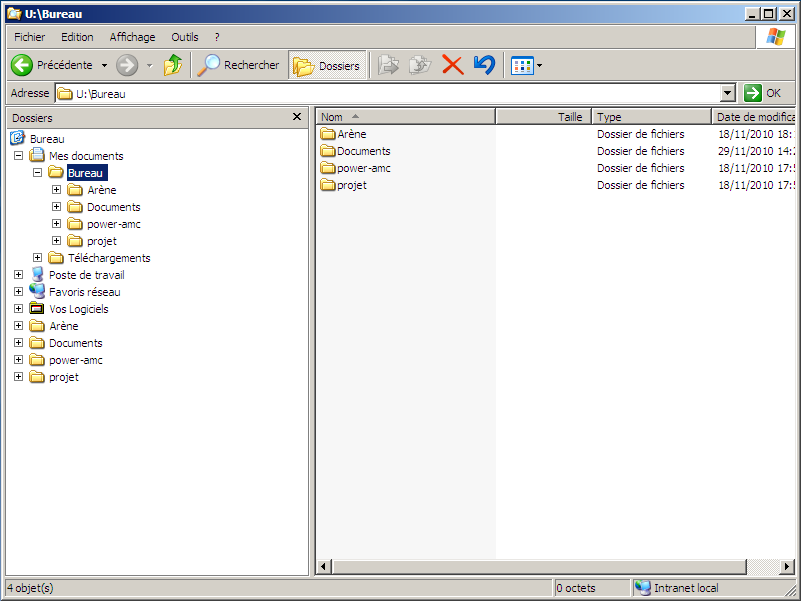
\includegraphics[height=2cm]{img/s02/explorer_windows.png}
        \end{center}
        \begin{center}
          Ligne de Commande\\
          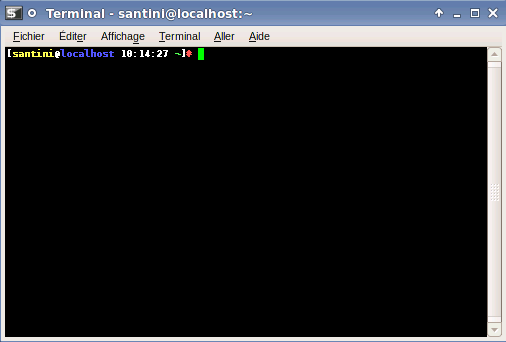
\includegraphics[height=2cm]{img/s02/terminal_single.png}
        \end{center}
      \end{block}
    \end{column}
    \begin{column}{75mm}
      \begin{block}{Boîte à outils : manipuler l'arborescence}
        \begin{center}
          \begin{tabular}{ll}
            \hline
            Commande&Fonction principale\\
            \hline
            \lin{pwd}&Afficher le nom du répertoire courant\\
            \lin{cd}&Changer de répertoire courant\\
            \lin{ls}&Afficher le contenu d'un répertoire\\
            \lin{cat}&Afficher le contenu d'un fichier\\\hline
            \lin{touch}&Créer un fichier\\
            \lin{mkdir}&Créer un répertoire\\\hline
            \lin{rm}&Supprimer fichier(s) ou répertoire(s) \\
            \lin{cp}&Copier fichier(s) ou répertoire(s)\\
            \lin{mv}&Déplacer/Renommer fichier(s) ou répertoire(s)\\
            \hline
          \end{tabular}
        \end{center}
      \end{block}
    \end{column}
  \end{columns}
\end{frame}
\manpage{pwd} \manpage{cd}
\manpage{ls} \manpage{ls(bis)} \manpage{cat}
\manpage{touch} \manpage{mkdir} \manpage{mkdir(bis)}
\manpage{rm} \manpage{rm(bis)} \manpage{cp}
\manpage{cp(bis)} \manpage{cp(ter)} \manpage{mv} \manpage{mv(bis)}
\manpage{mv(ter)}
\manpage{tar}\manpage{tar(bis)}

\begin{exercice}
  \begin{exercicelet}{Préparation}
    \begin{questions}
    \item Ouvrez un terminal. Vérifiez que le répertoire dans lequel
      vous êtes est bien \lin{/home/usager/123456789/}. Quelle est la
      commande qui permet de le faire ? (123456789 = votre identifiant)
    \item Vérifiez le contenu du répertoire \lin{Documents} qui est dans
      votre répertoire personnel. Quelle est la commande qui permet de
      le faire ? Est-ce qu'il y a quelque chose ?
    \item Faites la vérification de trois façons différentes : chemin
      absolu, utilisation du raccourci \lin{\~}, utilisation d'un chemin
      relatif.
    \item Changez le répertoire courant pour aller dans
      \lin{Documents}. Quelle est la commande pour le faire ?
    \item Créez en ligne de commande un répertoire \lin{m1101} dans
      \lin{\~/Documents}. À partir de maintenant, assurez-vous que le
      répertoire courant est ce répertoire \lin{m1101}.
    \item Téléchargez l'archive contenant les données pour ce TP:
      Allez sur la page
      \url{http://lipn.fr/~dubacq/m1101.html}.
      Téléchargez le fichier \lin{photos.tar}. Recherchez où
      le fichier a été écrit dans l'arborescence de votre répertoire
      personnel.
    \item Donnez la (suite de) commande(s) permettant de déplacer le
      fichier d'archive dans le répertoire \lin{m1101} que vous venez de
      créer. À la fin des commandes, le répertoire \lin{m1101} sera
      toujours votre répertoire courant et ne contiendra que le fichiers
      photos.tar.
    \item Quelle commande permet de vérifier que l'archive est bien dans
      le répertoire \verb|~/Documents/m1101|?
    \end{questions}
  \end{exercicelet}
\end{exercice}
\begin{exercice}
  \begin{exercicelet}{Examen de fichiers}
    \begin{questions}
    \item Quelles sont les informations données par le nom du fichier?
    \item\label{qsee} Les commandes \texttt{less}, \texttt{cat} et \texttt{hexdump} permettent
      d'afficher le contenu d'un fichier. Analysez la différence de
      comportement entre ces deux commandes sur le fichier
      \lin{photos.tar}. Qu'en concluez-vous? Quel est le programme le
      plus adapté pour voir le contenu de ce fichier ?
      \begin{correction}
        cat affiche brutalement du binaire sans filtrer
        (incompréhensible), less propose une interface (mais ça reste du
        binaire dans la configuration par défaut de Debian), hexdump
        transforme le binaire en hexadécimal (ce n'est pas beaucoup plus
        lisible). Le programme le plus adapté est donc... tar, comme
        montré dans la question suivante ! Avec \texttt{tar tf
          photos.tar} on obtient la liste des fichiers.
      \end{correction}
    \item Relisez le manuel de la commande \texttt{tar}. Vérifiez la
      liste des fichiers contenus dans l'archive. Combien y en a-t-il ?
    \item Sortez les fichiers de l'archive.
      \begin{correction}
        tar xf photos.tar
      \end{correction}
    \item Avec les commandes de la question~\ref{qsee}, regardez le
      fichier contenu dans un répertoire. Analysez la différence de
      comportement entre ces commandes. Qu'en concluez-vous?
      \begin{correction}
        La commande less est plus adaptée (pagination, arrêt par la
        touche q). La commande hexdump continue de produire de
        l'hexadécimal (on peut montrer hexdump -C aux curieux).
      \end{correction}
    \end{questions}
    
    Remarques: si un affichage prend trop de temps, utilisez le
    raccourci clavier adéquat pour suspendre l'exécution de la commande
    courante.  Si l'affichage de votre terminal est durablement
    perturbé, dans le menu Terminal \textrightarrow Réinitialiser le
    terminal.
  \end{exercicelet}
\end{exercice}
\subsection{Métacaractères}
\begin{frame}{Le métacaractère \lin{*}}
  \begin{block}{Le caractère \lin{*}}
    \begin{itemize}
    \item[\ddialogsystem] Le shell traduit la ligne de commande en \texttt{commande argument1
        argument2 ...}. Avant l'exécution, il traduit certains caractères
      selon des règles précisées ici.
    \item Le cataractère \lin{*} est utilisé comme un \textit{joker}
      pour remplacer une chaîne de caractères,
    \item Il est utilisé dans un chemin pour pointer plusieurs fichiers
      ou répertoires existants dont le chemin partage un motif commun.
    \item Le caractère \lin{*} peut être n'importe où dans le chemin,
      plusieurs fois si nécessaire.
    \end{itemize}
  \end{block}
  \begin{block}{Exemple de manipulation avec la commande \lin{mv}}
    \scriptsize{
      \begin{columns}
        \begin{column}{6cm}
          \begin{center}
            \mpromptS{%
              \promptS{mv *.jpg Images/}{} }
          \end{center}
        \end{column}
        \begin{column}{6cm}
          Ici, le chemin \lin{*.jpg} pointe tous les fichiers du
          répertoire courant dont le nom se fini par l'extension
          \lin{.jpg}. Il pointe donc les fichiers \lin{etacentauri.jpg}
          et \lin{aldebaran.jpg} et exclue les autres fichiers (ici le
          fichier \lin{alphacentauri.gif}).
        \end{column}
      \end{columns}
      \begin{columns}
        \begin{column}{6cm}
          \dirtree{%
            .1
            \DTd{{\color{solarizedRed}moi}}\DTfcomment{{\color{solarizedRed}Répertoire
                Courant}}.  .2 aldebaran{\color{solarizedGreen}.jpg}
            \DTfcomment{{\color{solarizedGreen}Fichier ciblé}}.  .2
            alphacentauri.gif .  .2
            etacentauri{\color{solarizedGreen}.jpg}
            \DTfcomment{{\color{solarizedGreen}Fichier ciblé}}.  .2
            \DTd{{\color{solarizedBlue}Images}}\DTfcomment{{\color{solarizedBlue}Répertoire
                final}}.  }
        \end{column}
        \begin{column}{6cm}
          \dirtree{%
            .1
            \DTd{{\color{solarizedRed}moi}}\DTfcomment{{\color{solarizedRed}Répertoire
                Courant}}.  .2 alphacentauri.gif .  .2
            \DTd{{\color{solarizedBlue}Images}}\DTfcomment{{\color{solarizedBlue}Répertoire
                final}}.  .3 {\color{solarizedGreen}aldebaran.jpg}
            \DTfcomment{{\color{solarizedGreen}Fichier déplacé}}.  .3
            {\color{solarizedGreen} etacentauri.jpg}
            \DTfcomment{{\color{solarizedGreen}Fichier déplacé}}.  }
        \end{column}
      \end{columns}
    }
  \end{block}
\end{frame}
\begin{frame}{Exemples d'utilisation de l'étoile}
  \begin{block}{Utilisation simple avec la commande \lin{mv}}
    \scriptsize{
      \begin{columns}
        \begin{column}{6cm}
          \begin{center}
            \mpromptS{%
              \promptS{mv al* Images/}{} }
          \end{center}
        \end{column}
        \begin{column}{6cm}
          Ici, le chemin \lin{al*} pointe tous les fichiers du
          répertoire courant dont le nom commence par les caractères
          \lin{al}. Il pointe donc les fichiers \lin{aldebaran.jpg} et
          \lin{alphacentauri.gif} et exclue les autres fichiers (ici le
          fichier \lin{etacentauri.jpg}).
        \end{column}
      \end{columns}
      \begin{columns}
        \begin{column}{6cm}
          \dirtree{%
            .1
            \DTd{{\color{solarizedRed}moi}}\DTfcomment{{\color{solarizedRed}Répertoire
                Courant}}.  .2 {\color{solarizedGreen}al}debaran.jpg
            \DTfcomment{{\color{solarizedGreen}Fichier ciblé}}.  .2
            {\color{solarizedGreen}al}phacentauri.gif
            \DTfcomment{{\color{solarizedGreen}Fichier ciblé}}.  .2
            etacentauri.jpg.  .2
            \DTd{{\color{solarizedBlue}Images}}\DTfcomment{{\color{solarizedBlue}Répertoire
                final}}.  }
        \end{column}
        \begin{column}{6cm}
          \dirtree{%
            .1
            \DTd{{\color{solarizedRed}moi}}\DTfcomment{{\color{solarizedRed}Répertoire
                Courant}}.  .2 etacentauri.jpg .  .2
            \DTd{{\color{solarizedBlue}Images}}\DTfcomment{{\color{solarizedBlue}Répertoire
                final}}.  .3 {\color{solarizedGreen}aldebaran.jpg}
            \DTfcomment{{\color{solarizedGreen}Fichier déplacé}}.  .3
            {\color{solarizedGreen}alphacentauri.gif}
            \DTfcomment{{\color{solarizedGreen}Fichier déplacé}}.  }
        \end{column}
      \end{columns}
    }
  \end{block}
  \begin{block}{Utilisation double avec la commande \lin{mv}}
    \scriptsize{
      \begin{columns}
        \begin{column}{6cm}
          \begin{center}
            \mpromptS{%
              \promptS{mv *centauri* JPG/}{} }
          \end{center}
        \end{column}
        \begin{column}{6cm}
          Ici, le chemin \lin{*centauri*} pointe tous les fichiers du
          répertoire courant dont le nom contient la chaîne de
          caractères \lin{centauri}. Il pointe donc les fichiers
          \lin{alphacentauri.gif} et \lin{etacentauri.jpg} et exclue les
          autres fichiers (ici le fichier \lin{aldebaran.jpg}).
        \end{column}
      \end{columns}
      \begin{columns}
        \begin{column}{6cm}
          \dirtree{%
            .1
            \DTd{{\color{solarizedRed}moi}}\DTfcomment{{\color{solarizedRed}Répertoire
                Courant}}.  .2 aldebaran.jpg .  .2
            alpha{\color{solarizedGreen}centauri}.gif
            \DTfcomment{{\color{solarizedGreen}Fichier ciblé}}.  .2
            eta{\color{solarizedGreen}centauri}.jpg
            \DTfcomment{{\color{solarizedGreen}Fichier ciblé}}.  .2
            \DTd{{\color{solarizedBlue}Images}}\DTfcomment{{\color{solarizedBlue}Répertoire
                Final}}.  }
        \end{column}
        \begin{column}{6cm}
          \dirtree{%
            .1
            \DTd{{\color{solarizedRed}moi}}\DTfcomment{{\color{solarizedRed}Répertoire
                Courant}}.  .2 aldebaran.jpg .  .2
            \DTd{{\color{solarizedBlue}Images}}\DTfcomment{{\color{solarizedBlue}Répertoire
                final}}.  .3 {\color{solarizedGreen}alphacentauri.gif}
            \DTfcomment{{\color{solarizedGreen}Fichier déplacé}}.  .3
            {\color{solarizedGreen}etcentauri.jpg}
            \DTfcomment{{\color{solarizedGreen}Fichier déplacé}}.  }
        \end{column}
      \end{columns}
    }
  \end{block}
\end{frame}
\begin{frame}{Métacaractère et chemins ciblés}
  \begin{block}{Exemple plus complexe et détails de l'interprétation}
    \begin{itemize}
    \item Le cararctère \lin{*} est développé lors de l'interprétation.
    \end{itemize}
  \end{block}
  \begin{center}
    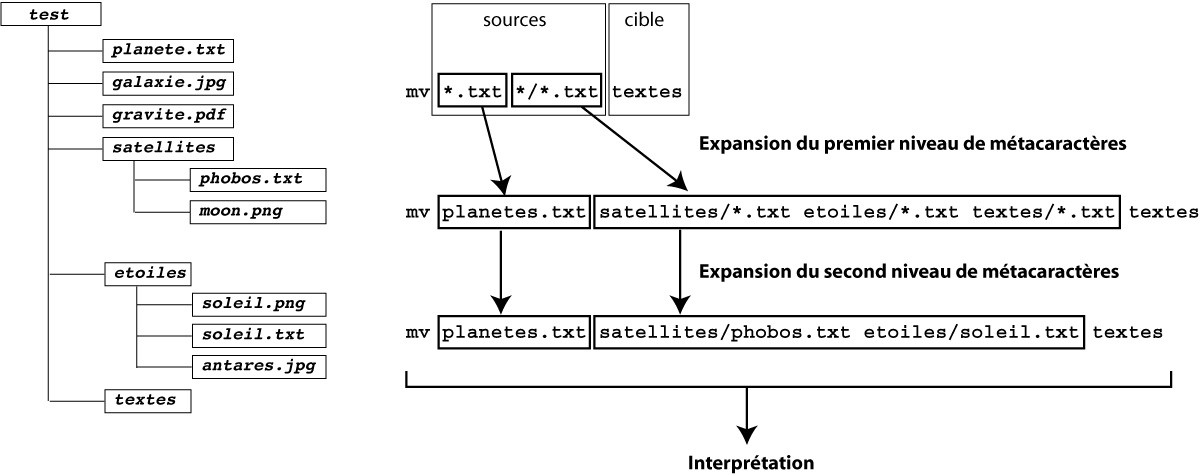
\includegraphics[width=12cm]{img/s02/star_met_mv_interp.jpg}
  \end{center}
\end{frame}
\begin{frame}{Autres métacaractères}
  \begin{alertblock}{Du shell aux programmes}
    Il faut bien se souvenir que les métacaractères sont interprétés par le shell. Cela a deux conséquences :
    \begin{itemize}
    \item Le programme appelé ne sait pas si les noms ont été tapés en entier ou si des métacaractères ont été utilisés. Il n'a que le résultat final.
    \item Dans un programme, on ne peut pas utiliser les métacaractères.
    \end{itemize}
  \end{alertblock}
  \begin{block}{Les jokers}
    Ce sont des motifs simples. Lorsqu'ils ne peuvent pas être
    instanciés, ils ne sont pas supprimés, mais passés tels
    quels. Exemple : \lin{mkdir -p toto/*} selon que \texttt{toto} est
    un répertoire non-vide ou autre chose.

    On y trouve \lin{?} qui remplace une lettre, \lin{[a-c][0-2]} qui remplace a0 b0 c0 a1 b1 c1 a2 b2 c2, 

  \end{block}
  \begin{block}{Les raccourcis}
    Le motif \lin{\{fourch,brou\}ette} est remplacé par
    \lin{fourchette} et \lin{brouette} indépendamment de
    l'existence ou nom de chemins correspondants.
    
    Le motif \lin{\~} a déjà été vu et est remplacé par le chemin absolu
    du répertoire personnel de l'utilisateur courant. \lin{\~{}user} est
    remplacé de la même façon mais pour l'utilisateur \emph{user}.
  \end{block}
\end{frame}
\begin{exercice}
  \begin{exercicelet}{Copie et déplacement}
    \begin{questions}
    \item Quelle commande permet la création "simultanée" de trois
      répertoires \lin{GIF} et \lin{Photos/Portugal},
      \lin{Photos/Marseille} et \lin{Photos/Montagne} ?
    \item Quelle commande permet de \emph{déplacer} depuis le répertoire
      \lin{images} tous les fichiers présentant l'extension
      \lin{gif} dans le répertoire \lin{GIF} nouvellement créé?
    \item Quelle commande permet de \emph{copier} depuis le répertoire
      \lin{images} tous les fichiers présentant l'extension
      \lin{jpg} dans le répertoire \lin{Photos} nouvellement créés?
    \item Définissez le répertoire \lin{Photos/Montagne} comme votre répertoire
      courant. Quelle commande permet de déplacer la photo de chalet dans ce répertoire ?
    \item En vous mettant dans \lin{Photos}, déplacez les photos
      restantes dans le bon répertoire (Marseille est supérieure à
      2000). Si possible, faites usages de jokers.
    \end{questions}
  \end{exercicelet}
\end{exercice}
\begin{exercice}
  \begin{exercicelet}{Suppressions}
    \begin{questions}
    \item Quel est le résultat de la séquence de commandes suivante :
\begin{verbatim}
 cd ..
 rm images
\end{verbatim}
    \item Comment modifier la dernière commande pour supprimer le
      répertoire \texttt{images/}? Comment modifier la commande pour
      éviter les invites de confirmation?
    \item Quelle commande permet de copier le répertoire \texttt{GIF} et
      son contenu dans un répertoire nommé \verb|images_GIF|?
    \item Quelle est la différence entre les deux commandes suivantes:
\begin{verbatim}
      cd ~
      cd /home/usager/votre_identifiant/
\end{verbatim}
    \item Fabriquez une archive qui contient le répertoire Photos (et
      uniquement celui-ci). Vérifiez son contenu.
    \end{questions}
  \end{exercicelet}
\end{exercice}
